\section{Introduction to Exact string matching}

\subsection{Problem introduction}

A very desirable feature in many search engines is to support queries of the form "Which documents contain the entire sentence 'X Y Z'?", instead of only searching for a single word or prefix of a word at a time. This create a new challenge for the search engine, as the best data structure is now unclear. 

Since a user might search for a sentence of arbitrary length, a first approach might be to simply store all possible sentences and then look up in which documents they appear. This, however, is a very bad idea and would require an enormous amount of space, as there are too many possibilities for every possible sentence. 

Other approaches might for each word store its context, such that the local environment (i.e. part of the sentence) could be looked up in the index. An example of this could be to store each word together with its next two words in a triple. If the size of the query sentence was upper bounded by a constant $O(1)$, this would be a good solution. However, for a query of unknown length, the index could never store enough local information to support every possible query. 

\kommentar{Nævn at suffix træer er en mulighed men at vi har valgt at prioritere andet}

This leaves the search engine with one way of looking up words: go back to the original text documents and use a string matching algorithm to find the sentence. How to decide which documents to look through is an important decision as it determines the total size of the search text. This will be discussed in section \ref{sec:index10}. 

\subsection{Naive search}

There exist many different algorithm for string matching, each with different strengths and weaknesses depending on the use case. Notable mentions are the Knuth-Morris-Pratt (KMP), Boyer-Moore, Rabin Karp, Aho-Corasick, and Apostolico–Giancarlo algorithms (the latter two being extensions of the first two). 

What are the differences betwween these algorithms and which ones are suitable for the problem of searching for a few occurences of a sentence of a couple of words in a text in the English language? 

To be able to compare various string matching algorithms, it is useful to have a baseline. A naive search method for string matching is described in algorithm \ref{alg:naivematch}. For each character in the text $T$, this algorithm uses $O(|P|)=O(n)$ time which results in $O(m\cdot n)$ total time. 

\begin{algorithm}[t]
\caption{Naive string matching algorithm}\label{alg:naivematch}
\begin{algorithmic}
\State Align $P$ to the left end of $T$.
\State Match each character in $P$ with the corresponding character in $T$ until a mismatch occurs.
\State If no mismatch occurs, report an match at the given position.
\State Increment the alignment of $P$ by one and repeat until $T$ is exhausted. 
\end{algorithmic}
\end{algorithm}

The way to achieve a speed-up to run in linear time, $(O(m+n)$, all algorithms use some sort of knowledge of either the pattern or the text to either shift $P$ by more than one character at a time or completely skip characters in $T$ if a match is not possible for some section. Before explaining the precise algorithms, an illustration of this can be helpful. 

Consider the text T=\verb|XABXYABXYABXZ| of length 13 and the pattern P=\verb|ABXYABXZ| of length 8. Following an example with notation from Gusfield\cite{Gusfield1997AlgorithmsOS}, the naive algorithm can be compared to two smarter possible versions, see figure \ref{fig:stringmatchingexample}. 

\begin{figure}[t]
\begin{verbatim}
      0        1              0        1              0        1   
      1234567890123           1234567890123           1234567890123
   T: XABXYABXYABXZ        T: XABXYABXYABXZ        T: XABXYABXYABXZ
   P: ABXYABXZ             P: ABXYABXZ             P: ABXYABXZ     
      *                       *                       *            
       ABXYABXZ                ABXYABXZ                ABXYABXZ    
       ^^^^^^^*                ^^^^^^^*                ^^^^^^^*    
        ABXYABXZ                   ABXYABXZ                ABXYABXZ
        *                          ^^^^^^^^                   ^^^^^
         ABXYABXZ                                                  
         *                                                         
          ABXYABXZ                                                 
          *                                                        
           ABXYABXZ                                                
           ^^^^^^^^                                                
\end{verbatim}
    \caption{A visual example of matching the a pattern P with a text T, using the naive algorithm and two smarter versions. A star beneath a character indicates a mismatch and a caret a match. }
    \label{fig:stringmatchingexample}
\end{figure}

The naive algorithm starts by finding a mismatch. It then shifts $P$ by one position, immediately and matches the next seven characters before finding the next mismatch at position 9 in $T$. It then shifts $P$ by one position and finds a mismatch three times before finally matching the whole pattern. 

A smarter algorithm recognises that when position 8 of $P$ mismatches with position 9 of $T$, then the next three shifts must be mismatches as the first letter $A$ will not match before encountering the next $A$ in the text. It knows this because the next $A$ in $P$ does not occur before position 5, so the smarter algorithm can shift the pattern four positions to align the two $A$s. 

Likewise, an even smarter algorithm can recognise that when position 8 of $P$ mismatches with position 9 in $T$, it has already matched the substring $ABX$, which is also the first three characters in $P$. Therefore, it does not need to compare these characters again after shifting $P$, as is shown in the figure \ref{fig:stringmatchingexample} when the rightmost algorithm does not even compare $ABX$ after shifting. 


\begin{comment} % How to algorithm
\begin{algorithm}
\caption{An algorithm with caption}\label{alg:cap}
\begin{algorithmic}
\Require $n \geq 0$
\Ensure $y = x^n$
\State $y \gets 1$
\State $X \gets x$
\State $N \gets n$
\While{$N \neq 0$}
\If{$N$ is even}
    \State $X \gets X \times X$
    \State $N \gets \frac{N}{2}$  \Comment{This is a comment}
\ElsIf{$N$ is odd}
    \State $y \gets y \times X$
    \State $N \gets N - 1$
\EndIf
\EndWhile
\end{algorithmic}
\end{algorithm}
\end{comment}

\subsection{Preprocessing}
The key to how the algorithm can figure out how to shift the pattern multiple positions or which parts of the pattern it does not need to compare lies in analysing the pattern before beginning to match in what is called the preprocessing step. Here, information like which characters there are in the pattern and where, along with which substrings match a prefix of the pattern, is obtained. For example, knowing that the letter $A$ only appears in position 1 and 5 of the pattern and that the substring, $ABX$ in position 5-7 matches a prefix of the pattern in position 1-3. 

The time spent in the preprocessing step typically only takes linear time in the length of the pattern and typically results in the time for the search step being reduced to linear in the text $O(m)$. This is what makes preprocessing so powerful and is why all string matching algorithm use some form of preprocessing of the pattern, or sometimes the text itself, for achieving linear or better time. 

\subsection{The Z algorithm}
The Z algorithm is a simple yet important algorithm in string matching and is sometimes referred to as a fundamental preprocessing step.\cite{Gusfield1997AlgorithmsOS} The Z algorithm is used to preprocess a string $S$ and results in an array of $Z_i(S)$ values that alone can be used to do string matching in linear time but is also used in the preprocessing step of other algorithms like the Knuth-Morris-Pratt and Boyer-Moore algorithms. Sometimes it is the entire basic string matching algorithm that the array of $Z_i(S)$-values results in that is called the Z algorithm, but here Z algorithm refers only to finding the $Z_i(S)$ values. 

In the following, the Z algorithm and the definitions required to understand it are introduced. The Z algorithm is explained in detail, before explaining how it can be used for the (KMP???) and Boyer-Moore algorithms. 

First off, consider the definition of $Z_i(S)$ for a given string $S$. When the string is clear by context, $Z_i$ can be used instead of $Z_i(S)$. 

\begin{itemize}
    \item[] \textbf{Definition} Given a string $S$ and a position $i>1$ let $Z_i(S)$ denote the length of the longest substring of $S$ that starts at $i$ and matches a prefix of $S$. 
\end{itemize}

This means that $Z_i$ is how far a substring starting in position $i$ can be read while matching the beginning of $S$. There is a nice way of visualising the $Z_i$ values for a given string, namely $Z$-boxes. Consider figure \ref{fig:z_boxes}, where the string $S$ is represented by a long horizontal line and for each position $x$ up to $i$ where $Z_x>0$, the substring starting at $x$ of length $Z_x$ is shown as a box. In this manner, each box represents a substring that matches a prefix of $S$. 

For a given position $i$, there may be many $Z$-boxes starting at a position less than $i$, so it is useful to have the following two definitions:

\begin{itemize}
    \item[] \textbf{Definition} For any position $i>1$ where $Z_i>0$ the $Z$-box at $i$ is defined as the substring starting at $i$ of length $Z_i$, ending in position $i+Z_i-1$. 
    \item[] \textbf{Definition} For every $i>1$, $r_i$ is the right-most endpoint of the \textit{$Z$-boxes} that begin at or before position $i$ and $l_i$ is the left end of one such $Z$-box. If there are more than one option, $l_i$ can refer to any one of them. 
\end{itemize}

\begin{figure}[t]
    \centering
    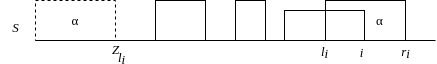
\includegraphics[width=.9\textwidth]{LaTeX/Figures/Zalg/zboxes.png}
    %\includesvg{LaTeX/Figures/Zalg/Zalg.drawio(1)}
    \caption{The solid boxes represent a substring of $S$ that matches a prefix of $S$, called $Z$-boxes. For a given position $i$, the right-most end of any $Z$-box beginning at or before $i$ is defined as $r_i$, the substring in that $Z$-box is $\alpha$, and the left end is $l_i$. }
    \label{fig:z_boxes}
\end{figure}

These definitions are enough to define and understand the Z algorithm. The Z algorithm works inductively by assuming for a position $i$ that the algorithm has correctly computed the $Z_x$ values for $x$ from 2 up to $i-1$ as well as the $r_{i-1}$ and $l_{i-1}$ values. It uses these to compute the next $Z_i$, $r_i$ and $l_i$ values. The idea is to use the concept of Z-boxes to infer information about the next $Z_i$ value and thus compute every $Z_i$ value in linear time. 

The Z algorithm divides into four different cases, which are most easily understood by following figure \ref{fig:Zalg}. 

Even though $r_i$ and $l_i$ are defined for each position $i$, the algorithm requires only the right-most $r$ value and its corresponding $l$ value and updates them when finding a $Z$-box that ends at a later position. This is why the algorithm uses a single variable to denote $r$ and $l$. 

\begin{algorithm}
\caption{Z algorithm}\label{alg:z_alg}
\begin{algorithmic}
\State Initialise $r=l=0$ and $Z_i=0$ for all $i$. 
\State For each position $k$, compute $Z_k$ and update $r$ and $l$ as follows
\For{$k=2..|S|$}
\If{$k>r$} \Comment{Case 1}
    \State Compute $Z_k$ explicitly by comparing characters from position $k$ to the \State beginning of $S$ until a mismatch is found. 
    \State $Z_k:=length\_of\_match$
    \State $l:=k$
    \State $r:=k+Z_k-1$
\ElsIf{$k\leq r$}
    \State Let $k':=l-k+1$ and $\beta:=S[k..r]$
    \If{$Z_{k'}<|\beta|$} \Comment{Case 2a}
        \State $Z_k:=Z_{k'}$
        \State $r$ and $l$ unchanged. 
    \ElsIf{$Z_{k'}>|\beta|$} \Comment{Case 2b}
        \State $Z_k:=|\beta|$
        \State $r$ and $l$ unchanged. 
    \ElsIf{$Z_{k'}=|\beta|$} \Comment{Case 2c}
        \State The substring $\beta$ matches a prefix of $S$ but might match longer than $Z_{k'}$. \State Match characters of $S$ from position $|\beta|+1$ with position $r+1$ until a \State mismatch occurs, say at position $q\geq r+1$. Then update
        \State $Z_k:=q-k$
        \State $r:=q-1$
        \State $l:=k$
    \EndIf
\EndIf
\EndFor
\end{algorithmic}
\end{algorithm}


\begin{figure}[t]
\centering
\begin{subfigure}{0.9\textwidth}
    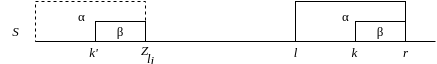
\includegraphics[width=\textwidth]{LaTeX/Figures/Zalg/Zalg1.png}
    \caption{The substring $S[k..r]$, labelled $\beta$, also occurs at position $k'$ of $S$}
    \label{fig:Zalg1}
\end{subfigure}
\hfill
\begin{subfigure}{0.9\textwidth}
    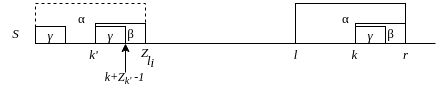
\includegraphics[width=\textwidth]{LaTeX/Figures/Zalg/Zalg2a.png}
    \caption{Case 2a. The longest substring, $\gamma$, starting at $k'$ matching a prefix of $S$ is shorter than $\beta$. }
    \label{fig:Zalg2a}
\end{subfigure}
\hfill
\begin{subfigure}{0.9\textwidth}
    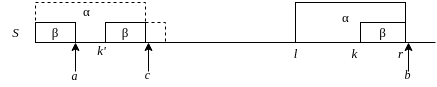
\includegraphics[width=\textwidth]{LaTeX/Figures/Zalg/Zalg2b.png}
    \caption{Case 2b. The longest substring starting at $k'$ matching a prefix of $S$ extends beyond the $Z$-box, meaning character $b$ and $c$ and thus $a$ and $b$ are a mismatch. }
    \label{fig:Zalg2b}
\end{subfigure}
\hfill
\begin{subfigure}{0.9\textwidth}
    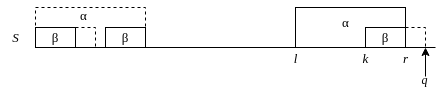
\includegraphics[width=\textwidth]{LaTeX/Figures/Zalg/Zalg2c.png}
    \caption{Case 2c. The length of longest substring starting at $k'$ matching a prefix of $S$ is exactly the length of $\beta$, meaning the match could extend further than $r$. }
    \label{fig:Zalg2c}
\end{subfigure}
\caption{The various cases of the Z algorithm. }
\label{fig:Zalg}
\end{figure}

\subsubsection{Explanation of the Z algorithm}
In order to work inductively, the algorithm must start by computing the first values for $Z_k$, $r$ and $l$. This is covered in case 1, where it explicitly compares $S[2..|S|]$ with $S[1..|S|]$ until a mismatch is found. In general, case 1 ensures that when position $k$ is not inside an already found $Z$-box, the algorithm will look for new boxes, not missing any. 

There are several cases when position $k$ is inside a $Z$-box. Denote the substring in the $Z$-box by $\alpha=S[l..r]$, which matches a prefix of $S$. This means character $S(k)$ matches position $k'=k-l+1$ of $S$. Similarly, the substring $\beta=S[k..r]$ matches the substring $S[k'..Z_l]$, see figure \ref{fig:Zalg1}. Logically, the substring beginning at position $k$ must then match a prefix of $S$ at least the minimum of $|\beta|$ and $Z_{k'}$. 

When $Z_{k'}<|\beta|$, called case 2a in the algorithm, the smaller substring $\gamma=S[k'..k'+Z_{k'}-1]$ is a maximal length substring that matches a prefix of $S$ and therefore the substring starting at position $k$ can match exactly $Z_{k'}$ characters at the beginning of $S$. 

When $Z_{k'}>|\beta|$, called case 2b in the algorithm, $\beta$ matches all characters in $S[k'..Z_l]$, but $S(|\beta|+1)=:a$ cannot match $S(k+|\beta|+1)=:b$. Why? Because by definition, $\alpha$ is a maximal length substring that matches a prefix of $S$, which means that there must be a mismatch at the end of the $Z$-box starting at position $l$ with the character at position $Z_l+1$, $c:=S(Z_l+1)$. And since $Z_{k'}>|\beta|$, the character $c$ matches the character $a$. Altogether this means that $a=c$ and $c\neq b$ implies $a\neq b$, i.e. that $S(|\beta|+1)$ mismatches $S(k+|\beta|+1)$. In this case, $Z_k=Z_{k'}$ and no more. 

Following the logic above, when $Z_{k'}=|\beta|$, the substring $\beta$ matches $S[k'..Z_l]$. But now $Z_{k'}=|\beta|$ only implies that $S(Z_{k'}+1)$ mismatches $S(k'+Z_{k'}+1$, i.e. $a\neq c$. From above, $c\neq b$ still holds, but now $a=b$ is a possibility, so start matching from those two characters beyond the current $Z$-box $\alpha$. When the next mismatch is found at position $q\geq r+1$, update $Z_k$, $r$ and $l$ as described in the algorithm, since a new right-most $Z$-box has been found. 

\subsection{More advanced string matching algorithms}

Using the Z algorithm, a basic algorithm that runs in linear time is apparent: given a pattern $P$ and text $T$, find all $Z_i$ values in $P\$T$ where $\$$ is a character not in the alphabet. All values are at most $n=|P|$ and when a position $i$ has $Z_i=n$, then the substring starting at $i$ in $P\$T$ matches $P$. This basic algorithm runs in linear time, since the Z algorithm runs in linear time. A proof for the linear time complexity of the Z algorithm is given in \cite{Gusfield1997AlgorithmsOS}. 

There exist many more advanced string matching algorithms than this basic one and these will be explored in the following. 

\section{Knuth-Morris-Pratt Algorithm}
The Knuth-Morris-Pratt (KMP) algorithm is a string-matching algorithm that efficiently searches for occurrences of a pattern within a larger text. It utilises a preprocessing step to build a partial match table, also known as the failure function. The failure function allows the algorithm to skip unnecessary comparisons during the matching process, resulting in improved performance.

The failure function built in the preprocessing step stores the lengths of the longest proper prefixes of $P$ that are also suffixes of the pattern up to each position $P[1..i]$. It is used to determine the number of characters to skip in the pattern when a mismatch occurs during matching and can be calculated in linear time using either a direct approach or the Z algorithm. 

Before searching the pattern is placed such that the first character of the pattern aligns with the first character of the search text. The first characters that are compared are the first character of the pattern and of the search text. 

If the characters match, the next character of the pattern and of the search text is compared, as KMP uses a left-to-right scan. 
If a mismatch occurs, the algorithm uses the information stored in the failure function to determine the next position to compare in the pattern. If the Failure function at the position of the mismatch in the pattern is greater than zero, it means that there is a prefix of the pattern of a length given in the Failure function, that is also a suffix of the substring matched until that point. In such cases, the pattern shifts such that the mismatched character of the search text aligns with the index of the pattern given by the failure function of the position of the mismatched character of the pattern.

The process continues until either a complete match is found, or if there is no text left to search in. If a match is found, the algorithm can either continue searching for additional occurrences or stop and return the index where the match starts.

By utilising the failure function to determine the number of characters to skip, the KMP algorithm avoids unnecessary comparisons and achieves a linear time complexity in the worst case, making it highly efficient for string-matching tasks.

\section{Boyer-Moore}

\subsection{Intro to Boyer Moore}
The key components in the Boyer-Moore algorithm are the right-to-left scan, the Bad Character Rule and the Good Suffix rule, which play a crucial role in improving the search process, as they are methods used to determine the amount by which a pattern can be shifted to the right during a search. By utilising the Good suffix rule and the Bad Character Rule, the algorithm reduces the number of unnecessary comparisons and skips larger portions of the search text. This allows the algorithm to avoid reading the entire text and in the best case achieve a sub-linear running time of $\Omega(m/n)$, thus performing better than KMP in the best case. The Boyer-Moore algorithm runs in $O(m)$ time when the pattern does not appear in the text and in general $O(n\cdot m)$ when the pattern does appear. The case where one is only interested in finding the first occurrence of a pattern is the same as when the pattern does not appear in the text: $O(m)$. Additionally, the Apostolico-Giancarlo extension of the algorithm makes it a $O(m)$ time in all cases. 

\subsection{Right to left scan}
In contrast to the naive methods, which use a left-to-right scan, the Boyer-Moore algorithm uses a right-to-left scan. Firstly the pattern is placed such that the first character of the pattern aligns with the first character of the search text. The first characters that are compared are however the most right character of the pattern and the aligned letter of the text. If it is a match it continues to compare the characters to the left. If it is a mismatch the patterns moved according to the Bad Character Rule or the Good Suffix Rule. If the whole pattern is matched, it is shifted again according to the Good Suffix Rule, which could be 1 position. The running time is hence $O(n\cdot m)$, as it in the worst case needs to match the whole pattern for each character of the text. An example of this worst case is when both the text and the pattern consist of the same repeated character, where Boyer-Moore becomes effectively identical to the Naive algorithm and makes exactly $n(m-n+1)$ comparisons. With the Apostolico-Giancarlo extension however, the algorithm matches and/or mismatches each character in the text at most once, resulting in at most $2m$ comparisons and giving $O(m)$ in all cases. 

\subsection{The Bad Character Rule}
There exists an Extended Bad Character Rule besides the Bad Character Rule. The original Boyer-Moore Algorithm only used the Bad Character Rule. This chapter will introduce both of them and in section \ref{sec:goodsuffixvsbadcharacter} it will be proven that the Extended Bad Character rule is obsolete when combined with the Good Suffix Rule. 

\subsubsection{The Bad Character Rule}
When a mismatch occurs, between a character $c_p$ from the pattern and a character $c_t$ from the text, the Bad Character Rule reasons that the pattern can be shifted, so that the rightmost occurrence of $c_t$ in the pattern matches $c_t$ in the text, if the occurrence is placed to the left of the mismatch. If the rightmost occurrence is placed on the right of the mismatch, the Bad Character Rule can only shift the pattern once. If no occurrences of $c_t$ exist in the pattern then the patterns can be shifted to the left until there no longer is an overlap of the pattern and $c_t$. 

\subsubsection{The Extended Bad Character Rule}
Extended Bad Character Rule is the addition that not only the right-most occurrence of a character is kept, but all occurrences, so the pattern can be shifted until the next time the character $c_t$ occurs. If the mismatch happens at the most left character of the pattern, the Bad Character Rule only allows shifting the pattern one step further.  If no occurrences of $c_t$ exist in the pattern then the patterns can still be shifted to the left until there no longer is an overlap of the pattern and $c_t$. 

\begin{figure}[t]
\begin{verbatim}
      0        1                  0        1             0        1      
      1234567890123456            12345678901            12345678901
   T: SomeBadCharacter         T: aabbabacdab         T: aabbabacdab
   P: BadCharacter             P: bacdab              P: bacdab          
                 *                   *^^                    *^^     
          BadCharacter             bacdab                   bacdab  
          ^^^^^^^^^^^^                                              
\end{verbatim}
\caption{Showing the bad character rule shifting successfully, the rule only shifting one position and the extended bad character rule being better in that case}
\label{fig:badcharacterrule_example}
\end{figure}

\subsubsection{R(x) values}
To calculate the number of characters the algorithm is allowed to skip, using the Bad Character Rule, without skipping the starting position of a potential match, the $R(x)$ values need to be introduced. 

\begin{itemize}
    \item[] \textbf{Definition} For each character in the alphabet, let $R(x)$ be the position of the rightmost occurrence of character $x$ in the pattern. $R(x)$ is defined to be zero if $x$ does not occur in $P$.
\end{itemize}

The $R(x)$ values can be calculated in $O(n)$ time using a hashmap. The hashmap has a key for every letter in the pattern and each key has a value representing at which position the rightmost occurrence of the letter is at. By iterating through the pattern from right to left, the position of a character in the pattern can be saved in the hashmap if the key, representing that letter, does not yet have a value. In this way, $R(x)$ is calculated in $O(n)$ time and is only using linear extra space in the size of the number of unique letters in the pattern.

%\kommentar{Figure om R(x) non extended values}

When using the Extended Bad Character Rule, it is not only the rightmost occurrence of character, that is necessary to save the position of, but all occurrences. This is because the pattern may be shifted to the rightmost occurrence of the $c_t$ to the left of a mismatch. Now it is necessary to use $R_i(x)$ values, which is the right-most occurrence of character $x$ in the pattern to the left of position $i$ and is defined to be zero if $x$ does not occur. A hashmap can still be used to keep of these $R_i(x)$ values, but the values of each key are now a list of positions in descending order. The lists are generated by iterating through the pattern from left to right, adding all positions of characters to the representative list in the hashmap. This still takes $O(n)$ time but now also uses $O(n)$ space.

%\kommentar{Figure om R(x) extended values}

With these definitions of $R(x)$ and $R_i(x)$ values, the Bad Character Rule and Extended Bad Character Rule can now be formally defined:

\begin{itemize}
    \item[] \textbf{Bad Character Rule} When a mismatch occurs at position $i$ in $P$ with character $x$ in $T$, look up the $R(x)$ value. If $R(x)<i$, then shift the pattern $i-R(x)$ positions so that $P(R(x))$ matches the $x$ in $T$ or the pattern is shifted beyond the $x$ if $R(x)=0$. If $R(x)>i$, then shift by one position. 
    \item[] \textbf{Extended Bad Character Rule} When a mismatch occurs at position $i$ in $P$ with character $x$ in $T$, shift $P$ by $i-R_i(x)$ positions, so $P(R_i(x))$ matches the $x$ in $T$ if $R_i(x)>0$, or the pattern is shifted beyond the $x$ if $R_i(x)=0$. 
\end{itemize}

\subsection{The Good Suffix rule}

\begin{figure}[t]
    \centering
    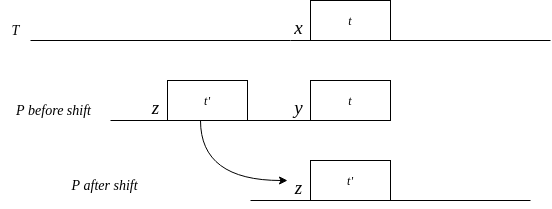
\includegraphics[width=\textwidth]{LaTeX/Figures/Zalg/suffixrule.png}
    \caption{Strong Good Suffix rule. The suffix $t$ matches but the next character mismatches $y\neq x$. Shift $P$ to the next time $t$ occurs with a different preceding character. }
    \label{fig:suffixrule}
\end{figure}

The Good Suffix rule is the other half of the Boyer-Moore algorithm and requires some more involved preprocessing. It is here that the Z algorithm can be used to more easily compute certain values and do so in linear time. There exist both a strong and a weak version of the Good Suffix rule, where the original Boyer-Moore only used the weak version\cite{Gusfield1997AlgorithmsOS}, but the strong version can make larger shifts with no added time or space. The following focuses on the strong version. 

\begin{itemize}
    \item[] \textbf{Strong Good Suffix Rule} When a suffix of $P$ has been matched with a substring $t$ of $T$ and a mismatch occurs at the next preceding character, then find in $P$ the right-most copy $t'$ of $t$ of in $P$ such that the character preceding $t'$ is different from the character preceding $t$ in $P$ ($z\neq y$ in figure \ref{fig:suffixrule}) and shift $P$ so that $t'$ in $P$ aligns with $t$ in $T$. If no such occurrence of $t'$ exists in $P$, shift $P$ by the least amount so that a prefix of $P$ aligns and matches a suffix of $t$ in $T$. If that is not possible, shift $P$ entirely past $t$ in $T$. 
    \item[] \textbf{Occurrence of P} When an occurrence of $P$ is found in $T$, shift $P$ by the least amount so that a prefix of $P$ aligns and matches a suffix of $P$ in $T$. If that is not possible, shift $P$ entirely past $P$ in $T$. 
\end{itemize}

In order to support this rule, some different values are to be computed from $P$ in the preprocessing step. These are called the $L'(i)$ and $l'(i)$ values. $L'(i)$ is used to find the occurrence of $t'$ in $P$ where $t=P[i..n]$, and $l'(i)$ is used to shift $P$ (by the least amount) so that a prefix of $P$ matches a suffix of $P[i..n]$. They are defined as follows:

\begin{itemize}
    \item[] \textbf{Definition} For each $i$, $L'(i)$ is the largest position less than $n$ such that the substring $P[i..n]$ matches a suffix of $P[1..L'(i)]$ and such that the character (if it exists) preceding that suffix is not equal to $P(i-1)$. $L'(i)$ is defined to be zero if there is no position satisfying the conditions. 
    \item[] \textbf{Definition} For each $i$, let $l'(i)$ denote the length of the longest suffix of $P[i..n]$ that is also a prefix of $P$. If none exists, $l'(i)$ is defined to be zero. 
\end{itemize}

Using a theorem from \cite{Gusfield1997AlgorithmsOS} (Theorem 2.2.2), the Z algorithm can be used to compute the $L'(i)$ values in linear time. This simply extends to computing the $l'(i)$ values as well. It works as follows:

Use the Z algorithm on the reversed string $P^r$. These values can be used to compute new $N_j(P)$ values defines as $N_j(P)=Z_{n-j+1}(P^r)$. Since $Z_i(S)$ is the length of the longest substring of $S$ that starts at $i$ and matches a prefix of $S$, $N_j(P)$ correspond to the length of the longest suffix of the substring $P[1..j]$ that is also a suffix of $P$. These values are, maybe unsurprising, very useful in finding the $L'(i)$ and $l'(i)$ values. 

Then it is clear that for each $i$, $L'(i)$ is the largest index $j$ less than $n$ such that $N_j(P)=|P[i..n]|=n-i+1$. Additionally, $l'(i)$ equals the largest $j\leq|P[i..n]|=n-i+1$ such that $N_j(P)=j$. 

Combining these results, the $L'(i)$ and $l'(i)$ values can be computed using the following algorithm:

\begin{algorithm}
\caption{Computing $L'(i)$ and $l'(i)$}\label{alg:Lvalues}
\begin{algorithmic}
\State Initialise $L'(i):=0$ and $l'(i):=0$ for all $i$. 
\For{$j=1..n-1$}
    \If{$N_j>0$}
        \State $i:=n-N_j+1$
        \State $L'(i):=j$
    \EndIf
\EndFor
\For{$j=1..n-1$}
    \If{$N_j=j$}
    \State $l'(n-j+1) := j$
    \Else
    \State $l'(n-j+1) := l'(n-j+2)$ \Comment{$l'(n+1)$ is defined to be $0$}
    \EndIf
\EndFor
\end{algorithmic}
\end{algorithm}

% Her er et eksempel som kan flyttes til hvor det passer bedst. 
\begin{figure}[h!]
\begin{verbatim}
                              0        1      
                              123456789012345 
                          S : tapftapgtapftap 
                          Nj: 00300070003000_ 
                          L': 000000007000b0_ 
                          l': _77777777333300 
\end{verbatim}
\caption{Example showing the values of $N_j$, $L'$, and $l'$ for the string $tapftapgtapftap$. The number $b$ means 11 and the symbol '$\_$' represents the value not being defined for that index. }
\label{fig:gsr-example}
\end{figure}


Finally, the Good Suffix rule can be defined more precisely using these values. 

\begin{itemize}
    \item[] \textbf{The Strong Good Suffix Rule with exact shifts} When a mismatch occurs at position $i-1$ of $P$, and $L'(i)>0$, then shift $P$ by $n-L'(i)$ positions. If $L'(i)=0$, meaning that $t'$ from figure \ref{fig:suffixrule} does not exist, shift the pattern by $n-l'(i)$ positions, which is the least amount so that a prefix of the shifted pattern matches a suffix of $t$. When an occurrence of $P$ is found, shift by $n-l'(2)$. These are correct even when $l'(i)=0$. In the case that the mismatch occurs at position $n$, then shift by only 1 position. 
\end{itemize}


\subsubsection{Interaction between the Good Suffix and the Extended Bad Character rule}\label{sec:goodsuffixvsbadcharacter}

As explained, the whole Boyer-Moore algorithm uses both the Bad Character rule and the Good Suffix rule to determine how far to shift the pattern without missing a possible occurrence in the text. An interesting nontrivial fact is that when using the Good Suffix rule, the Extended Bad Character rule will actually never be better than using just the Bad Character rule. More formally,

\begin{itemize}
    \item[] \textbf{Lemma 1} When a mismatch occurs in position $i$ of $P$ with a character $x$ in $T$ and $x$ occurs in $P$ to the right of position $i$, the Good Suffix rule will always shift $P$ more than the Extended Bad Character rule, making the Extended Bad Character Rule no better than the regular Bad Character rule. 
\end{itemize}

\begin{figure}[t]
    \centering
    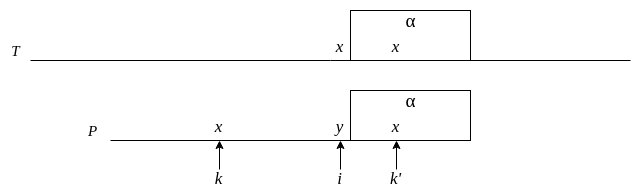
\includegraphics[width=\textwidth]{LaTeX/Figures/Zalg/suffixvsbadchar.png}
    \caption{The suffix $\alpha$ of $P$ matches with $T$ until mismatching character $x$ in $T$ at position with position $i$ in $P$. The next $x$ to the left of position $i$ occurs at position $k$ and the next $x$ to the right at position $k'$.}
    \label{fig:suffixvsbadchar}
\end{figure}

\subsubsection{Proof}

Let $\alpha=P[i+1..|P|]$ be the suffix of $P$ that has matched a substring of $T$ until the mismatch. Since it is assumed that $x$ occurs in $\alpha$, let $k'$ be the left-most position of such an $x$. Further, let $k$ be the position of the right-most $x$ in the prefix $P[1..i-1]$ - if no such $x$ exists, $k$ is defined to be zero. See figure \ref{fig:suffixvsbadchar}. 

Since the mismatching character occurs in $P$ to the right of the mismatch, the regular Bad Character Rule gives no information and could only shift $P$ by one position, so this is the only case where the extended rule would be used. The Extended Bad Character rule would shift $P$ to the right until the next occurrence of $x$ matches with the mismatched $x$ in $T$. Thus, the Extended Bad Character Rule will shift $P$ by $i-k$ positions, also when $k=0$. 

The Good Suffix Rule looks for an occurrence of $\alpha$ in $P$. First assume $k=0$. Then $\alpha$ does not occur again in $P$, and the Good Suffix rule will shift $P$ by $n-l'(i+1)$. In general, $l'(j)$ for any $j$ is at most $n-j+1$, but since $x$ does not occur in $P$ to the left of $k'$, then $l'(i+1)$ will be at most $n-k'$ and the Good Suffix rule will shift by at least $n-(n-k') = k'$ positions. 

If $k>0$, then either the substring $\alpha$ matches the $x$ in position $k'$ with $x$ around position $k$, that is, at $S[k-(k'-i)+1\ ..\ k-(k'-i)+1+|\alpha|]$, or $\alpha$ matches at a position more to the left (or $\alpha$ does not match at all, shifting as mentioned above). This is because it is not possible for $\alpha$ to match a position where $k'$ would be shifted to the right of $k$ since, by construction, there is no occurrence of $x$ strictly between position $k$ and $k'$. This means the Suffix rule will shift by at least $k'-k$ in this case. 

Altogether, the Good Suffix rule will shift by at least $k'$ or $k'-k$ positions, both of which are larger shifts than $i-k$ from the Extended Bad Character rule. 

\rightline{$\square$}

\subsection{The whole Boyer-Moore algorithm}

The Boyer-Moore algorithm uses both the Bad Character rule and 



\subsection{Apostolico-Giancarlo}


\section{Full text Indexes}\label{sec:index10}
Four Indexes where generated to support full-text searching.

\subsection{Index 10.0 and 10.1}
The Indexation of indexes 10.0 and 10.1 is exactly like in index 8: A hash map where each unique word has a key, and the value of each key is an Article list, representing which articles the word is present in. The indexing time is therefore still linear. However, the search functions differ, as these indexes support full-text indexing.

When searching for a query, The article list for each word in the query is looked up and the intersection of the article list is calculated. This takes $O(tri_q\cdot a)$ time as looking up $tri_q$ articles list in the hash table takes $O(tri_q\cdot a)$ time and performing $tri_q - 1 $ AND operations to calculate the intersection takes $O(tri_q\cdot a)$ time.

All the articles that contain all of the words of the query are then searched through to find the exact match of the query using KMP in index 10.0 and Boyer-Moore in 10.1. Both algorithms run in linear time. 

\subsection{Index 11.0 and 11.1}
The Indexation of indexes 11.0 and 11.1 does not hash individual words when indexing, like index 10, but rather triples of continuous words in a string. 

\textbf{Definition} A triplet of a sentence is three continuous words in the sentence. There are thereby n-2 triplets in a sentence.

When searching for a query, The article list for each triplet of the query is looked up and the intersection of the article list is calculated. These indexes thereby used $O(tri_t\cdot a)$ space, where a is the number of articles and $tri_t$ is the number of unique triplets in a text. Technically, t is upper bounded by $O(u^3)$ (where u is upper bounded by $O(n)$) as there could be all possible configurations of triplets. This poor space complexity should especially be considered if the nature of a search text is prone to contain all possible combinations of triplets of unique words (eg if DNA basepairs were considered as words and the full text were a long DNA string).  $O(u^3)$ is here considered to be an overestimation when considering an English text. It is therefore that the variable $tri_t$ is introduced.

The search function in Index 11.0 simply returns the intersection as the result. This result may be incorrect as it is possible that all triplets of a query exist in a text but not in one continuous sequence. This search function is however very fast as it simply needs to look up $tri_q$ articles list, where $tri_q$ is the number of triplets in the query, and find the intersection of these queries. This takes $O(tri_q\cdot a)$ time as looking op $tri_q$ articles list in the hash table takes $O(tri_q\cdot a)$ time and performing $tri_q - 1 $ AND operations to calculate the intersection takes $O(tri_q\cdot a)$ time.

The search function in index 11.1 searches through all the articles that contain all of the triplets of the query, using Boyer-Moore. This gives an exact result and is predicted to be much faster than index 10, as many articles may be excluded, making the total search string much smaller. The factor of the reduction of the search string depends tremendously on the content of the query and the search text.